\chapter{Наблюдатель пониженного порядка}
\label{ch:chap4}

\section{Условие задачи}

Рассмотреть систему:
$$
  \begin{cases}
    \dot{x} = Ax + Bu \\
    y = Cx + Du
  \end{cases}
$$ и выполнить следующие шаги:

    \begin{itemize}
    \item Найти собственные числа матрицы A и определить управляемость и наблюдаемость каждого из них. 
    Сделать вывод об управляемости, стабилизируемости, наблюдаемости и обнаруживаемости системы.
    \item Построить схему моделирования системы, замкнутой регулятором, состоящем из наблюдателя состояния 
    $\dot{\hat{x}} = A\hat{x} + (B+LD)u + L(C\hat{x} - y)$ и закона управления $u = K\hat{x}$.
    \item Задаться парой достижимых желаемых спектров для регулятора и наблюдателя,
    обеспечивающих асимптотическую устойчивость замкнутой системы.
    \item Синтезировать регулятор $K$ на основании выбранного желаемого спектра, опре
    делить собственные числа матрицы $(A+BK)$ и сравнить с желаемым спектром
     для проверки корректности расчетов.
    \item Синтезировать матрицу коррекции наблюдателя $L$ на основании выбранного же
    лаемого спектра, определить собственные числа матрицы $(A +LC)$ и сравнить с
     желаемым спектром для проверки корректности расчетов.
     \item  Выполнить моделирование с начальными условиями системы
     $x(0) = \begin{bmatrix} 1 & 1 & 1 & 1\end{bmatrix}^T$ и наблюдателя 
     $\hat{x}(0) = \begin{bmatrix} 0 & 0 & 0 & 0 \end{bmatrix}^T$. Построить графики 
     формируемого регулятором управления $u(t)$, сравнительные графики $x(t), \hat{x}(t)$,
     а также ошибки наблюдателя $e(t) = x(t) - \hat{x}(t)$.
    
    
    \end{itemize}


\section{Решение задачи}

Параметры для объекта:
$$
  A = \begin{bmatrix}
    5 & -7 & -5 & 1 \\
    -7 & 5 & -1 & 5 \\
    -5 & -1 & 5 & 7 \\
    1 & 5 & 7 & 5
  \end{bmatrix} \tab
  B = \begin{bmatrix}
    5\\7\\1\\9
  \end{bmatrix}^T \tab
  C = \begin{bmatrix}
    0 & 1 & 0 & 0 \\
    1 & 0 & 0 & 0 
  \end{bmatrix}^T \tab
  D = \begin{bmatrix}
    4\\2
  \end{bmatrix} 
$$

\subsection{Исследование характеристик системы}
Найдём собственные числа матрицы $A$:
$$
    \sigma(A) = \{-8, 4, 8, 16\}
$$
Чтобы не вычислять матрицу Хаутусу для наблюдаемости/управляемости каждого собственного числа, для начала проверим по матрице наблюдаемости/управляемости полные характеристики:
$$
  V = \begin{bmatrix}
    C \\
    CA \\
    CA^2 \\
    CA^3
  \end{bmatrix} \tab 
  U = \begin{bmatrix}
    B & AB & A^2B & A^3B 
  \end{bmatrix}
$$
$$
  rank(V) = 4, \tab rank(U) = 4
$$
Матрицы вышли полноранговыми, а значит наша система полностью наблюдаема/управляема по всем собственным числам и в целом. 
Стабилизируемость/обнаруживаемость также следует из прошлого вывода.

\subsection{Синтез наблюдателя}

Для наблюдателя пониженного порядка, то есть наблюдателя не за всеми компонентами вектора состоянии нашей системы, выберем следующие матрицы $Y, G$:
$$
  G = \begin{bmatrix}
    -3 & 1 \\
     0 & -3 
  \end{bmatrix}, \tab
  Y = \begin{bmatrix}
    1 & 0 \\
    0 & 1
  \end{bmatrix}
$$
Очевиден её спектр: $\sigma(G) = \{-3, -3\}$. Условия на синтез наблюдателя будут теми же, что и для полного порядка, просто оперировать будем матрицами меньшими размерностями.

Получим матрицу преобразования $Q$, решив уравнения Сильвестра:
$$
  GQ - QA = YC, \tab \rightarrow \tab Q = \begin{bmatrix}
    0.03 &  -0.03  &  0.09  & -0.07 \\
   -0.02 &   0.05  &  0.07  & -0.09
  \end{bmatrix}
$$

Как и в случае с полным порядком, пропускаем выход объекта и управления через динамическую систему с матрицей $G$ и получаем что-то полезное:
$$
  \begin{aligned}
    \dot{z} = QAQ^{-1}z + QBu, \\
    \dot{\hat{z}} = G\hat{z} - Yy + (QB+YD)u
  \end{aligned}
$$
Для управления по обратной связи нам понадобится вектор состояния, вот как он будет формироваться:
$$
    u = K\hat{x}, \tab \hat{x} = \begin{bmatrix}
                        C\\Q
                      \end{bmatrix}^{-1} \begin{bmatrix}
                        y - Du \\ \hat{z}
                      \end{bmatrix}
$$

\begin{figure}[ht]
  \centering
  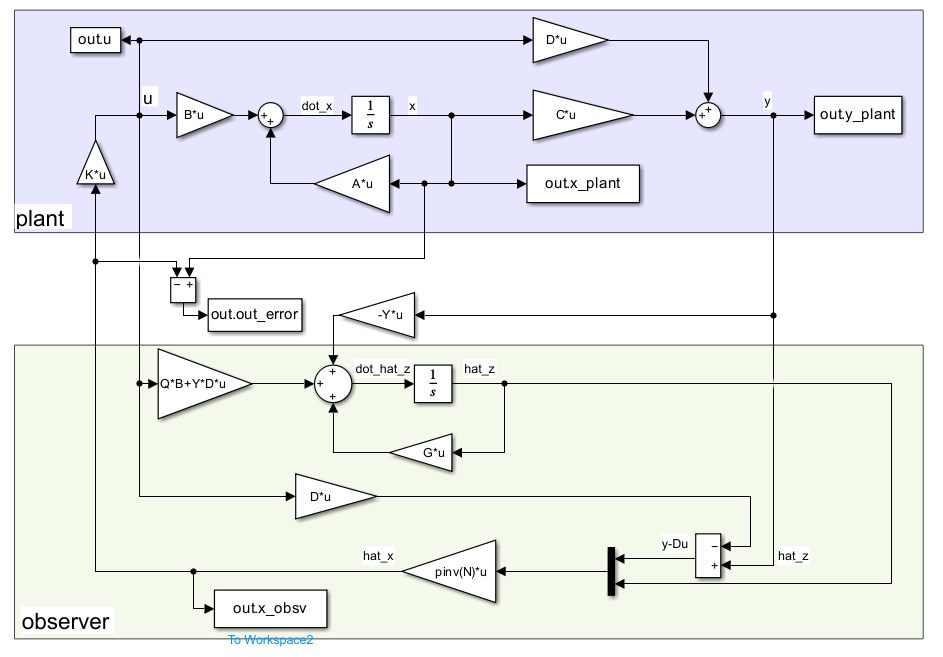
\includegraphics[width=0.8\textwidth]{model_observer_down_controller.png}
  \caption{Схема наблюдателя пониженного порядка с обратной связью по управлению}
\end{figure}

\newpage
\subsection{Синтез регулятора}

Для синтеза регулятора воспользуемся матрицами $Y,G$ из прошлого задания, коэффициенты регулятора идентичны\dots
$$
K = 
\begin{bmatrix}
  8.51 & -8.91 & -0.87 & -1.36
\end{bmatrix}
$$

\subsection{Моделирование}
Выполним моделирование с начальными условиями системы 
$x(0) = \begin{bmatrix} 1 & 1 & 1 & 1\end{bmatrix}^T$ и наблюдателя 
$\hat{x}(0) = \begin{bmatrix} 0 & 0 & 0 & 0 \end{bmatrix}^T$:
Как можно заметить, ошибка наблюдателя почти сразу становится предельна мала, 
поэтому на векторе состояние наблюдатель почти сразу сливается с компонентами вектора состояния\dots


\begin{figure}[ht]
  \centering
  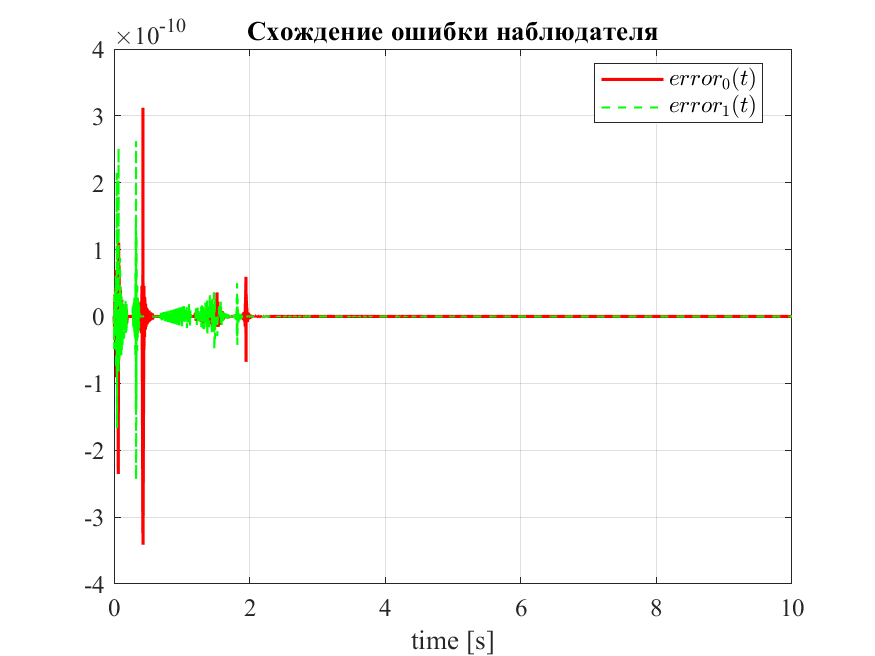
\includegraphics[width=0.8\textwidth]{low_dim_error1.png}
  \caption{Ошибка наблюдателя}
\end{figure}
\newpage
\begin{figure}[ht]
  \centering
  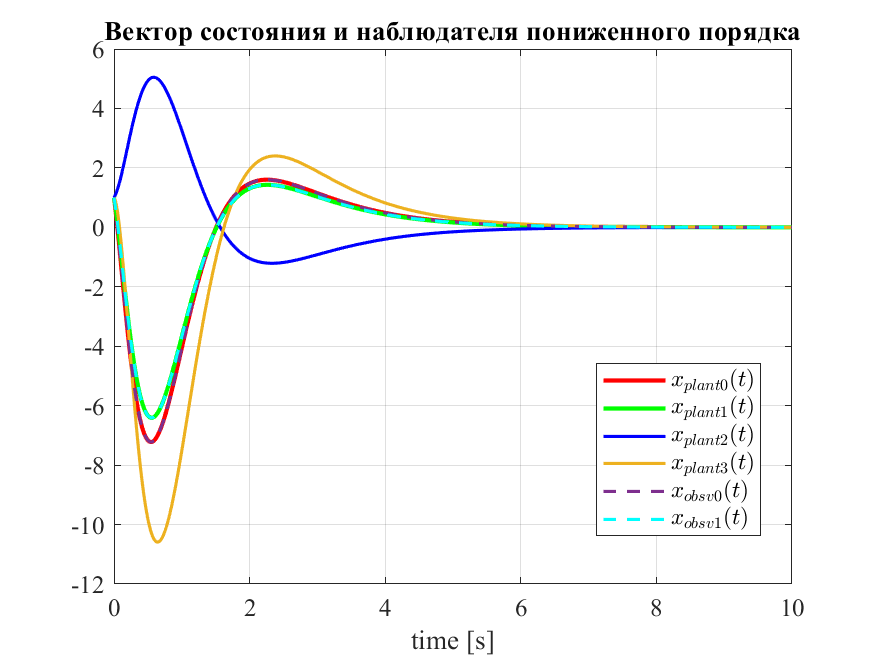
\includegraphics[width=0.8\textwidth]{low_dim_compare1.png}
  \caption{Состояния системы - сравнение}
\end{figure}
\begin{figure}[ht]
  \centering
  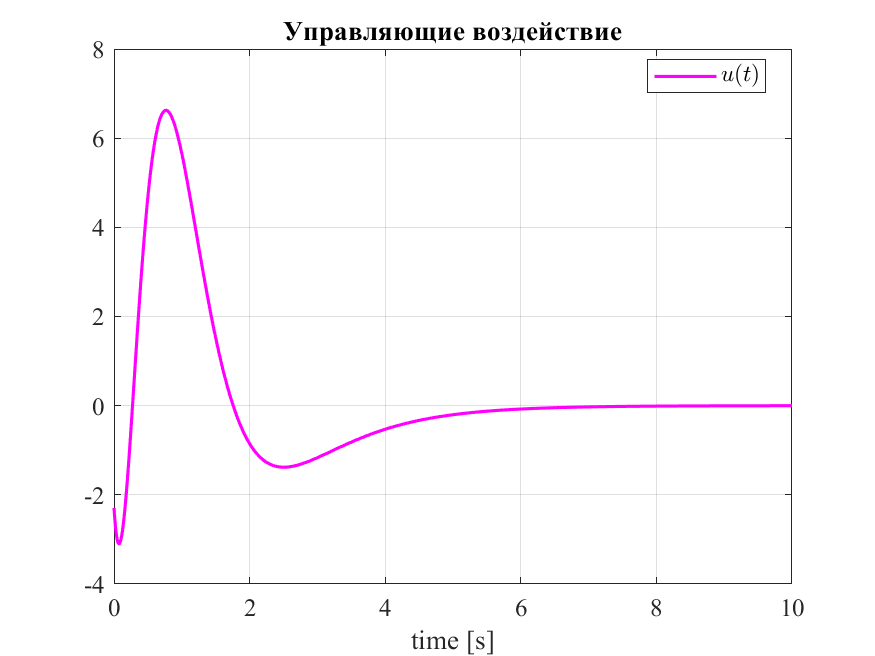
\includegraphics[width=0.8\textwidth]{low_dim_u1.png}
  \caption{Управление регулятора}
\end{figure}
\newpage
\subsection{Вывод}

В этом задании мы синтезировали связку модального наблюдателя пониженного порядка и регулятора. 
Здесь мы работали с полностью наблюдаемой и управляемой системой, поэтому мы могли использовать любой желаемый спектр у наблюдателя/регулятора.
При моделировании мы отслеживали всего лишь 2 компоненты состояния системы, хотя она состоит из 4-х, 
для этого мы использовали другой подход к синтезу наблюдателя, но по прежнему основанный 
на решение уравнения Сильвестра, который нам позволил найти матрицу преобразования $Q$. 

Моделирование показало, что связка отработала успешно.

\endinput
